\documentclass[10pt, a4paper]{article}
\usepackage[T1]{fontenc}
\usepackage[english]{babel}
\usepackage[margin=1cm]{geometry}
\usepackage[utf8]{inputenc}
\usepackage{fontawesome}
\usepackage{graphicx}
\usepackage{hyperref}
\usepackage{natbib}
% List spacing
\usepackage{enumitem}
% Source Sans Pro font
\usepackage{sourcesanspro}
\renewcommand{\familydefault}{\sfdefault}
% Headings format 
\usepackage{titlesec}

\renewcommand{\bibsection}{\section*{Publications}}
\bibliographystyle{plainnat}
% Disable page number
\pagenumbering{gobble}

 
% Paragraph spacing
\newcommand{\parspace}{0.3\baselineskip}
\newcommand{\parspaceshort}{0.3\baselineskip}
\newcommand{\parspaceveryshort}{0.1\baselineskip}
\usepackage[skip=\parspace]{parskip}
\makeatletter
\newcommand{\@minipagerestore}{\setlength{\parskip}{\parspace}}
\makeatother
% Headings
\titleformat*{\section}{\normalfont\large\bfseries}%\color{MidnightBlue}}
\titleformat*{\subsection}{\bfseries}%\color{MidnightBlue}}

% Title format
\makeatletter

\def\@maketitle{

\newpage


{\LARGE\textbf{{\@title}} \par}
May 4th, 1998 | \faMapMarker ~ Bologna, Italy

\href{mailto:kmfrick98@gmail.com}{\texttt{kmfrick98@gmail.com}}  | \url{https://kmfrick.tech}

\url{https://github.com/kmfrick} | \url{https://linkedin.com/in/kmfrick}

\hfill\smash{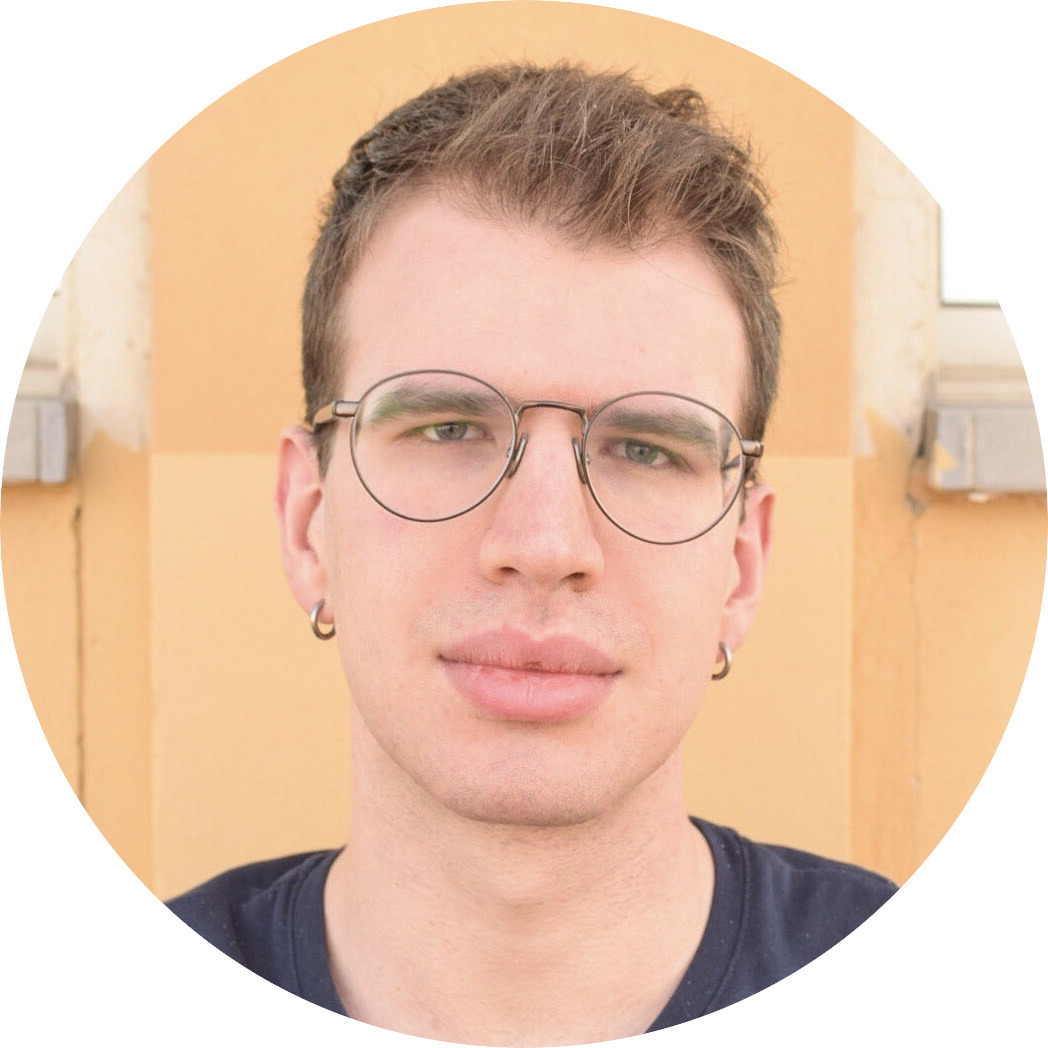
\includegraphics[width=3.5cm]{frickkm.JPG}}


}
\makeatother

% Headings spacing 
\titlespacing\section{0pt}{\parspace plus 2pt minus 2pt}{\parspace plus 2pt minus 2pt}
\titlespacing\subsection{0pt}{\parspace plus 2pt minus 2pt}{\parspace plus 2pt minus 2pt}

% List spacing
%\setlist{nosep, leftmargin=*}
\setlist{parsep=\parspaceveryshort, topsep=\parspaceveryshort, itemsep=\parspaceveryshort, leftmargin=*}

\title{Kevin Michael Frick}
\author{}

\begin{document}
  
\maketitle

\vspace{-0.8em}
\hrulefill
\vspace{0.8em}


%\begin{minipage}[t]{0.7\textwidth}
\section*{Work experience}
\textbf{Computer Science Teacher} | Istituto Tecnico Aldini Valeriani, Bologna, IT | 11/2020 - Present
\begin{itemize}
\item Teaching computer science theory, C++ programming fundamentals and simple data structures to students aged 16-17.
\item Teaching lab classes together with a technical/pratical teacher, following a problem-based approach that centers student learning around open-ended, student-driven problems.
\item Coordinating and teaching an optional course covering more advanced topics such as graph theory and dynamic programming, preparing students for the national selection for the International Olympiad in Informatics (IOI).
\end{itemize}
\textbf{Computer Vision Research Intern} | Robotics and Mechatronics, University of Twente, NL | 03/2020 - 06/2020
\begin{itemize}
\item Erasmus+ traineeship with the goal of improving the localization and mapping (SLAM) capabilities of an unmanned aerial vehicle through research and deployment of deep neural networks for semantic segmentation of 3D scenes.
\item Developed a module for the ROS framework able to integrate a state-of-the-art SLAM solution with neural networks that make use of TensorFlow's, TensorFlow Lite's and PyTorch's C++ and Python APIs.
\item Developed and deployed a Docker container that significantly reduced environment set-up times and compatibility issues.
\end{itemize}

\section*{Education}
\textbf{MSc Computer Engineering} | Collegio Superiore, University of Bologna, IT | 09/2020 - Present
\begin{itemize}
\item Honors program of the University of Bologna, offering advanced and interdisciplinary education by means of courses, seminaries and lectures concerning various topics from different fields. 
\item Admission depends on a selective test which is solely based on merit.
Seven BSc STEM students are admitted each year and are provided with a personal tutor, exemption from annual fees, free accommodation and an annual scholarship throughout their bachelor's and master's degrees.
\item Selected coursework: artificial intelligence and tuProlog programming, computer systems engineering and x86 assembly, information security and penetration testing, operating systems and concurrent programming in Go 1.15. Attending additional courses about mathematics, physics, economics, etc. at Collegio Superiore.
\item Student representative to the Network of Italian Students in Schools and Institutes for Higher Study (RIASISSU) from 2020 to 2022. Responsible for organizing and coordinating joint activities between the Collegio Superiore and other Italian honors colleges such as the Scuola Normale Superiore in Pisa. 
\end{itemize}
\textbf{BSc Computer Engineering} | Collegio Superiore, University of Bologna, IT | 09/2017 - 07/2020 | Summa Cum Laude, GPA: 29.6/30
\begin{itemize}
\item Thesis: "Machine Learning for Semantic Visual SLAM"
\item Selected coursework: C11 and Java 11 programming, Linux system programming, software engineering patterns and principles, statistical models and R programming,
computer networks, data engineering fundamentals and administration of DB2 databases, electronics and telecommunications. Attended additional courses about economics, physics, etc. at Collegio Superiore.
\end{itemize}
%\end{minipage}\hfill
%\begin{minipage}[t]{0.28\textwidth}

\section*{Languages}
Italian, native speaker | English, fluent, IELTS Academic 8.5
\section*{Honors and awards}
\begin{itemize}
\item Italian national selection for the International Olympiad in Informatics (IOI): \textbf{bronze medal} won in the 2016 final round of individual competitions, \textbf{third place} in the 2016 final round of team competitions.
\item European Union Science Olympiad (EUSO): \textbf{silver medal} in the 2014 national final round, tackling the physics challenge. 
\end{itemize}
%\end{minipage}

\section*{Projects}
\begin{itemize}
\item Game engine pathfinder: developed a pathfinding solution that is able to efficiently find optimal and collision-free paths for an arbitrary number of actors in an open source reimplementation of a computer role-playing game. Languages and libraries involved: C++11, Python 3, SDL, OpenAL.

\item OrarioSync: web application that allows users to download their college timetables and allow for phone calendar synchronization. Languages and frameworks involved: Python 3, ZEIT Now v2, JavaScript ES6, React.

\item Academic software engineering project: led a team of 3 people to detail an in-depth requirements, domain and risk analysis and develop a software solution to manage a bike rental service. Personally designed mock-ups of the UI using Figma. Languages and frameworks involved: Azure App Service, C\# 8.0, .NET Core 3.1, Azure SQL, Entity Framework Core, Bootstrap 4, jQuery.

\end{itemize}
\nocite{*}
\bibliography{CV}

\end{document}
